\documentclass[12pt]{exam}

\usepackage[utf8]{inputenc}  % For UTF8 source encoding.
\usepackage{amsmath}  % For displaying math equations.
\usepackage{amsfonts} % For mathematical fonts (like \mathbb{E}!).
\usepackage{upgreek}  % For upright Greek letters, such as \upvarphi.
\usepackage{wasysym}  % For additional glyphs (like \smiley!).
\usepackage{mathrsfs} % For script text (hash families and universes).
\usepackage{enumitem}
\usepackage{graphicx}
% For document margins.
\usepackage[left=.8in, right=.8in, top=1in, bottom=1in]{geometry}
\usepackage{lastpage} % For a reference to the number of pages.
\usepackage[table,xcdraw]{xcolor}
\usepackage{pdfpages}
\usepackage{verbatim}
\usepackage{afterpage}

\newcommand*{\authorname}{Luis A. Perez}

\newcommand*{\duedate}{Wednesday, August 7th}
\newcommand*{\duetime}{11:59 pm}

% Fancy headers and footers
\headrule
\firstpageheader{EE 263\\Summer 2019}{Homework 3 \\ }{Due: \duedate\\at \duetime}
\runningheader{EE 263}{Homework 6}{\authorname}
\footer{}{\footnotesize{Page \thepage\ of \pageref{LastPage}}}{}

% Exam questions.
\newcommand{\Q}[1]{\question{\large{\textbf{#1}}}}
\qformat{}  % Remove formatting from exam questions.

% Useful macro commands.
\newcommand*{\bigtheta}[1]{\Theta\left( #1 \right)}
\newcommand*{\bigo}[1]{O \left( #1 \right)}
\newcommand*{\bigomega}[1]{\Omega \left( #1 \right)}
\newcommand*{\prob}[1]{\text{Pr} \left[ #1 \right]}
\newcommand*{\ex}[1]{\text{E} \left[ #1 \right]}
\newcommand*{\var}[1]{\text{Var} \left[ #1 \right]}

\newcommand*{\norm}[1]{\left\lVert #1 \right\rVert}
\newcommand*{\HH}{\mathscr{H}}   % Family of hash functions.
\newcommand*{\UU}{\mathscr{U}}   % Universe.
\newcommand*{\eps}{\varepsilon}  % Epsilon.


% Custom formatting for problem parts.
\renewcommand{\thepartno}{\roman{partno}}
\renewcommand{\partlabel}{\thepartno.}

% Framed answers.
\newcommand{\answerbox}[1]{
\begin{framed}
\hspace{\fill}
\vspace{#1}
\end{framed}}

\printanswers

\setlength\answerlinelength{2in} \setlength\answerskip{0.3in}

\begin{document}
\title{EE 263 Homework 6}
\author{\authorname}
\date{}
\maketitle
\thispagestyle{headandfoot}
\setcounter{MaxMatrixCols}{15}

\begin{questions}
%%%%%%%%%%%%%%%%%%%%%%%%%%%%%%%%%%%
\Q{Optimal operation of a two-state chemical reactor}

  \begin{solution}
    \begin{enumerate}[label=(\alph*)]
      \item We have the dynamics equation $\dot{x}(t) = A_jx(t)$. This can be solved directly as the following:
      \[
        x(t) = e^{tA_j}x(0)
      \]
      If we operate the first reactor for $T_0$ time followed by the second reactor for $T - T_0$ time, our final state will be:
      \[
        x(T) = e^{(T - T_0)A_2}x(T_1) = e^{(T - T_0)A_2}e^{T_0A_1}x(0)
      \]
      With the above, we can now write a function $C_k(T_0)$ which will give us the amount of compounds $k$ at time $T$. We have:
      \[
        C_k(T_0) = e_k^Te^{(T - T_0)A_2}e^{T_0A_1}x(0)
      \]
      where $e_k$ is the $k$-th unit vector. Since our answer only needs to be accurate to two decimal places, computing the optimal value of $T_0$ that maximizes the above can be done through a simple search. We simply compute $C_k(t)$ for all $0 < t \leq T$ at intervals of of size $0.001$, and report the value $t_{\text{max}}$ which achieves the maximum $C_k$.
      \item
        We perform the method described above. See Figure \ref{fig:chemical_b} for plot. We conclude that:

        The optimal value is $T_0 = 0.61$ with $0.37$ units of compound 2 at time $T = 1$.

      \item
        We follow a similar set-up as before. In this case, the final state of the system will be given by:
        \[
          x(T) = e^{(T-T_2)A_1}e^{(T_2 - T_1)A_2}e^{T_1 A_1}x(0)
        \]
        We can similarly define a function for the $k$-th chemical as:
        \[
          C_k(T_1, T_2) = e_k^Te^{(T-T_2)A_1}e^{(T_2 - T_1)A_2}e^{T_1 A_1}x(0)
        \]
        Since we're once again only interested in a solution accurate up to 2 decimal places, we can just try suitable values of $T_1$ and $T_2$ in intervals of size $0.001$.

        \item
          We perform the method described above. See Figure \ref{fig:chemical_d} for plot. We conclude that:

          The optimal value is $T_1 = 0.49$ and $T_2 = 0.87$ with $0.38$ units of compound 2 at time $T = 1$.
    \end{enumerate}
  \end{solution}

  % \afterpage{\clearpage}
  \begin{figure}[hpb!]
    \centering
    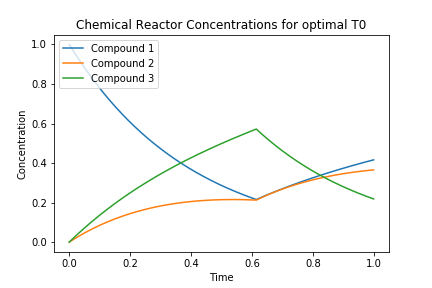
\includegraphics{chemical_reactor_b.png}
    \caption{Chemical concentrations for $T_0 = 0.61$ (part b)}
    \label{fig:chemical_b}
  \end{figure}
  
  \afterpage{\clearpage}
  \begin{figure}
    \centering
    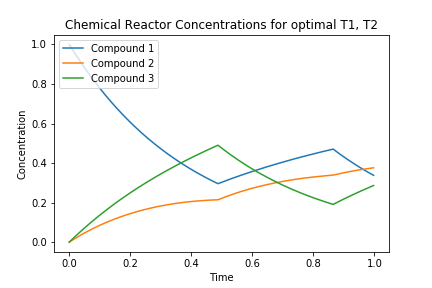
\includegraphics{chemical_reactor_d.png}
    \caption{Chemical concentrations for $T_1 = 0.49$ and $T_2 = 0.87$ (part d)}
    \label{fig:chemical_d}
  \end{figure}


  \newpage
  \Q{Harmonic Oscillator}
  \begin{solution}
    \begin{enumerate}[label=(\alph*)]
      \item We find the eigenvalues, resolvent, and state transition matrix for the matrix:
      \[
        A =
          \begin{bmatrix}
            0 & \omega \\
            -\omega & 0
          \end{bmatrix}
      \]
      The resolvent in our case is given by:
      \begin{align*}
        (sI - A)^{-1} = 
          \begin{bmatrix}
            s & -w \\
            w & s
          \end{bmatrix}^{-1} \\
          \frac{1}{s^2 + w^2}\begin{bmatrix}
            s & w \\
            -w & s
          \end{bmatrix}
      \end{align*}
      We can also derive the eigenvalues by simply solving:
      \begin{align*}
        \text{det}(A) = s^2 + w^2 = 0  \\
        \implies s = \pm iw \tag{Where $i = \sqrt{-1}$}
      \end{align*}
      From the above, we can compute the state transition matrix as:
      \[
        \Phi = 
          \begin{bmatrix}
            \cos \omega t & \sin \omega t \\
            -\sin \omega t & \cos \omega t
          \end{bmatrix}
      \]
      Finally, we can express $x(t)$ as:
      \[
        x(t) = \Phi x(0)
      \]
      \item
        The vector field is sketched out in Figure \ref{fig:vector_field_sketch}.
      \item
        We wish to verify that $||x(t)||$ is constant. Let's do this directly as:
        \begin{align*}
          ||x(t)|| &= \sqrt{x(t)^Tx(t)} \\
          &= \sqrt{x(0)^T\Phi^T\Phi x(0)} \\
          &= \sqrt{x(0)^T 
          \begin{bmatrix}
            \cos^2 \omega t + \sin^2 \omega t & -\cos \omega t \sin \omega  + \sin \omega t \cos \omega t \\
            \sin \omega t \cos \omega t  -\cos \omega t \sin \omega  & \sin^2 \omega t + \cos^2 \omega t
          \end{bmatrix}
          x(0)} \\
          &= \sqrt{x(0)^T 
          \begin{bmatrix}
            1 & 0 \\
            0 & 1
          \end{bmatrix}
          x(0)} \\
          &= \sqrt{x(0)^Tx(0)} \\
          &= ||x(0)||
        \end{align*}
        From the above, we can conclude that $||x(t)||$ is constant for all $t$.
      \item
        We verify directly that the velocity vector is always orthogonal to the position vector. Take $x \in \mathbb{R}^2$ to be some aribitray position. Then we have:
        \begin{align*}
          x^T\dot{x} &= x^T\begin{bmatrix} 0 & \omega \\ -\omega & 0 \end{bmatrix} x \tag{Given dynamics} \\
          &= \begin{bmatrix} x_1 & x_2 \end{bmatrix} \begin{bmatrix} 0 & \omega \\ -\omega & 0 \end{bmatrix} \begin{bmatrix} x_1 \\ x_2 \end{bmatrix} \\
          &= \begin{bmatrix} x_1 & x_2 \end{bmatrix} \begin{bmatrix} wx_2 \\ -wx_1 \end{bmatrix} \\
          &=  wx_1x_2 - wx_1x_2 \\
          &= 0
        \end{align*}
        As such, we conclude our proof.
    \end{enumerate}
  \end{solution}

  \begin{figure}[htbp]
    \centering
    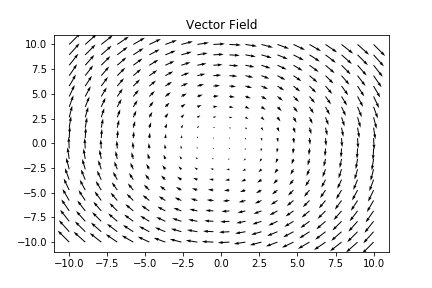
\includegraphics{vector_field_example.png}
    \caption{Vector Field Sketch for the Harmonic Oscillator}
    \label{fig:vector_field_sketch}
  \end{figure}

  \newpage
  \Q{Interconnection of linear systems}
  \begin{solution}
    Our task is to express the overall system (consisting of subsystems $S$ and $T$) as a single lineary dynamical systen with input, state, and output given by:
    \[
      \hat{u} = \begin{bmatrix}
        u \\ v
      \end{bmatrix},
      \hat{x} = \begin{bmatrix}
        x \\ z
      \end{bmatrix},
      \hat{y} = y
    \]
    This is actually relatively straight-forward. First, we need to express each of the equations of each sub-system as a linear combination of only $u,v,x,z$ and $y$. We begin with the dynamics equations:
    \begin{align*}
      \dot{x} &= Ax + B_1u + B_2w_1 \tag{Given dynamics of subsystem $S$} \\
      &= Ax + B_1u + B_2H_1z \tag{Using the fact that $w_1 = H_1z$} \\
      \dot{z} &= Fz + G_1v + G_2w_2 \tag{Given dynamics of subsystem $T$} \\
      &= Fz + G_1v + G_2(Cx + D_1u + D_2w_1) \tag{Using given formula for $w_2$} \\
      &= Fz + G_1v + G_2(Cx + D_1u + D_2H_1z) \tag{Using formula for $w_1$} \\
      &= (F + G_2D_2H_1)z + G_2Cx + G_1v + G_2D_1u \tag{Grouping like-terms}
    \end{align*}
    Note that we can express the equations above in matrix form as:
    \begin{align*}
      \begin{bmatrix}
        \dot{x} \\ \dot{z}
      \end{bmatrix} &= 
      \begin{bmatrix}
        A & B_2H_1 \\
        G_2C & F + G_2D_2H_1
      \end{bmatrix}
      \begin{bmatrix}
        x \\ z
      \end{bmatrix}
      + 
      \begin{bmatrix}
        B_1 & 0 \\
        G_2D_1 & G_1 
      \end{bmatrix}
      \begin{bmatrix}
        u \\ v
      \end{bmatrix}
    \end{align*}
    We can immediately tell from the above our dynamics and input matrix for the single lineary dynamical system.

    Next, we takle the output equation. We focus on expression $y$ as a function of $x,z, u$ and $v$.
    \begin{align*}
      y &= H_2z + Jw_2 \tag{Given output equation} \\
      &= H_2z + J(Cx + D_1u + D_2w_1) \tag{Equation for $w_2$} \\
      &= H_2z + J(Cx + D_1u + D_2H_1z) \tag{Equation for $w_1$} \\
      &= (H_2 + JD_2H_1)z + JCx + JD_1u \tag{Grouping like terms}
    \end{align*}
    We can rewrite the above in matrix form as:
    \[
      y =
        \begin{bmatrix}
          JC & H_2 + JD_2H_1
        \end{bmatrix}
        \begin{bmatrix}
          x \\ z
        \end{bmatrix}
        + 
        \begin{bmatrix}
          JD_1 & 0
        \end{bmatrix}
        \begin{bmatrix}
          u \\ v
        \end{bmatrix}
    \]
    From the above, we can immediately read off our output and feed-through matrices. We did not need to make any assumptions.

    However, to be extremely explicit, we have now written our system in the form:
    \begin{align*}
      \dot{\hat{x}} &= \hat{A}\hat{x} + \hat{B}\hat{u} \\
      \hat{y} &= \hat{C}\hat{x} + \hat{D}\hat{u}
    \end{align*}
    where:
    \begin{align*}
      \hat{x} &= \begin{bmatrix} x \\ z \end{bmatrix} \\
      \hat{u} & \begin{bmatrix} u \\ v \end{bmatrix}  \\
      \hat{y} &= y \\
      \hat{A} &= 
        \begin{bmatrix}
          A & B_2H_1 \\
          G_2C & F + G_2D_2H_1
        \end{bmatrix} \\
      \hat{B} &=
        \begin{bmatrix}
          B_1 & 0 \\
          G_2D_1 & G_1 
        \end{bmatrix} \\
      \hat{C} &= 
        \begin{bmatrix}
          JC & H_2 + JD_2H_1
        \end{bmatrix}\\
      \hat{D} &= 
        \begin{bmatrix}
          JD_1 & 0
        \end{bmatrix}
    \end{align*}
  \end{solution}

  \newpage 
  \Q{Analysis of investment allocation strategies}
  \begin{solution}
    \begin{enumerate}[label=(\alph*)]
      \item It turns out that both investment strategies can be described using essentially the same framework. However, for simplicity, we start with the $35-35-30$ strategy. We define our input state to be:
      \[
        x(t) =
          \begin{bmatrix}
            B_1(t) \\
            B_2(t) \\
            B_3(t) \\
            B_2(t-1) \\
            B_3(t-1) \\
            B_3(t-2)
          \end{bmatrix} \in \mathbb{R}^6
      \]
      Note that $B_i(t) = 0$ for $t < 0$. Our initial state is therefore:
      \[
        x(0) =
          \begin{bmatrix}
            0.35 \\ 0.35 \\ 0.30 \\ 0 \\ 0 \\ 0
          \end{bmatrix} \in \mathbb{R}^6
      \]
      We can immediately compute our total wealth at time $t$ as:
      \[
        y(t) = Cx(t) = w(t) = B_1(t) + B_2(t) + B_3(t) + B_2(t-1) + B_3(t-1) + B_3(t-2)
      \]
      where 
      \[
        C = \begin{bmatrix}
          1 & 1 & 1 & 1 & 1 & 1
        \end{bmatrix} \in \mathbb{R}^{1 \times 6}
      \]
      For the dynamics matrix, we have:
      \[
        x(t + 1) = Ax(t)
      \]
      where $A \in \mathbb{R}^{6 \times 6}$ is given by:
      \begin{align*}
        A &=
          \underbrace{\begin{bmatrix}
            0.35 \\
            0.35 \\
            0.30 \\
            0 \\
            0 \\
            0
          \end{bmatrix}
          \begin{bmatrix}
            1.05 & 0.06 & 0.07 & 1.06 & 0.07 & 1.07
          \end{bmatrix}}_{\text{Total payout is re-invested by purchasing new bonds}}
          + 
          \underbrace{
          \begin{bmatrix}
            0 & 0 & 0 & 0 & 0 & 0 \\
            0 & 0 & 0 & 0 & 0 & 0 \\
            0 & 0 & 0 & 0 & 0 & 0 \\
            0 & 1 & 0 & 0 & 0 & 0 \\
            0 & 0 & 1 & 0 & 0 & 0 \\
            0 & 0 & 0 & 0 & 1 & 0 
          \end{bmatrix}}_{\text{Update state for one time-step}} \\
          &= 
          \begin{bmatrix}
            0.3675 & 0.021 & 0.0245 & 0.371 & 0.0245 & 0.3735 \\
            0.3675 & 0.021 & 0.0245 & 0.371 & 0.0245 & 0.3735 \\
            0.315 & 0.018 & 0.021 & 0.318 & 0.021 & 0.321 \\
            0 & 1 & 0 & 0 & 0 & 0 \\
            0 & 0 & 1 & 0 & 0 & 0 \\
            0 & 0 & 0 & 0 & 1 & 0 
          \end{bmatrix}
      \end{align*}
      The easiest way to explain is in parts. The first summand when multiplied by $x(t)$ serves to compute the total payout at time $t$, and then re-distributes this payout by purchasing new bonds at $t+1$, $B_1(t+1), B_2(t+1), B_3(t+1)$. The second summand simply updates our state, since $B_i(t)$ is the ``the amount of $i$-year CDs boughts at period $t$'', and since one-time period is passing, these take the place of $B_i(t-1)$ in our state vector.


      With the above complete, we move on to the $60-20-20$ strategy. We use the same framwork as above, with just a few minor modifications. With this strategy, we have:
      \[
        x(0) = \begin{bmatrix} 0.6 \\ 0.2 \\ 0.2 \\ 0 \\ 0 \\ 0 \end{bmatrix}
      \]
      and we have:
       \begin{align*}
        A &=
          \underbrace{\begin{bmatrix}
            0.60 \\
            0.20 \\
            0.20 \\
            0 \\
            0 \\
            0
          \end{bmatrix}
          \begin{bmatrix}
            1.05 & 0.06 & 0.07 & 1.06 & 0.07 & 1.07
          \end{bmatrix}}_{\text{Total payout is re-invested by purchasing new bonds}}
          + 
          \underbrace{
          \begin{bmatrix}
            0 & 0 & 0 & 0 & 0 & 0 \\
            0 & 0 & 0 & 0 & 0 & 0 \\
            0 & 0 & 0 & 0 & 0 & 0 \\
            0 & 1 & 0 & 0 & 0 & 0 \\
            0 & 0 & 1 & 0 & 0 & 0 \\
            0 & 0 & 0 & 0 & 1 & 0 
          \end{bmatrix}}_{\text{Update state for one time-step}} \\
          &= 
          \begin{bmatrix}
            0.63 & 0.036 & 0.042 & 0.636 & 0.042 & 0.642 \\
            0.21 & 0.012 & 0.014 & 0.212 & 0.014 & 0.214 \\
            0.21 & 0.012 & 0.014 & 0.212 & 0.014 & 0.214 \\
            0 & 1 & 0 & 0 & 0 & 0 \\
            0 & 0 & 1 & 0 & 0 & 0 \\
            0 & 0 & 0 & 0 & 1 & 0 
          \end{bmatrix}
      \end{align*}
      The $C$ matrix remains the same.
      \item We want to understand the limit:
      \[
        \lim_{t \to \infty} \frac{w(t+1)}{w(t)}
      \]
      From the above, we know that:
      \[
        w(t) = Cx(t) = CA^tx(0)
      \]
      As such, we need to understand the limiting behavior of $A^tx(0)$. We recall from lecture the following formulation, for diagonalizable $A$ (we check that this is true for the 35-35-30 strategy):
      \[
        x(t) = A^tx(0) = \sum_{i=1}^6 \lambda_i^t(w_i^Tx(0)v_i) \tag{$A$ is diagonalize for 35-35-30 strategy}
      \]
      where $\lambda_i, w_i, v_i$ are the eignevalues, right, and left eigenvectors. As such, to understand the limiting behavior of $x(t)$ as $t \to \infty$, we need to compute these values for $A$.

      Doing this for the $35-35-30$ strategy, we have the absolute of the eigenvalues:
      \begin{align*}
        \lambda_1 &= 1.06265258 \\
        \lambda_2 &= -0.32657629 + 0.44206583j \\
        \lambda_3 &=  -0.32657629 - 0.44206583j \\
        \lambda_4 &= \lambda_5 = \lambda_6 = 0 
      \end{align*}
      As such, we can see that $\lambda_1$ will dominate as $t \to \infty$ (it has the largest absolute value). With this, we can simplify our ratio:
      \begin{align*}
        \lim_{t \to \infty} \frac{w(t+1)}{w(t)} &= \lim_{t \to \infty} \frac{CA^{t+1}x(0)}{CA^tx(0)} \\
        &= \lim_{t \to \infty} \frac{C \sum_{i=1}^6 \lambda_i^{t+1}(w_i^Tx(0)v_i)}{C\sum_{i=1}^6 \lambda_i^t(w_i^Tx(0)v_i)} \tag{Subtituting $A^tx(0)$} \\
        &=\lim_{t \to \infty} \frac{\lambda_1^{t+1}Cw_1^Tx(0)v_1 }{\lambda_1^{t}Cw_1^Tx(0)v_1}  \tag{As $t \to \infty$, only $\lambda_1$ survives} \\
        &= \lim_{t \to \infty} \frac{\lambda_1^{t+1}}{\lambda_1^{t}} \tag{Factor out and cancel values not dependent on $t$} \\
        &= \lambda_1
      \end{align*}
      As such, we have that the wealth ration is simply given by the dominant eigenvalue. In the case of the $35-35-30$ we have:
      \[
        \lim_{t \to \infty} \frac{w(t+1)}{w(t)} = \lambda_1 = 1.06265258 
      \]

      We would like to carry out a similar analysis for the 60-20-20 strategy. However, it turns out that the state matrix for this strategy is not diagonizable. As such, we must use the generilized Jordan Canonical form. In this case, we have:
      \[
        x(t) = A^tx(0) = \sum_{i=1}^4 T_iJ_i^t(S_i^Tx(0)) \tag{$A$ is not-diagonalize for 60-20-20 strategy}
      \]
      By a similar analysis for the case of the $60-20-20$ strategy, we have the eigenvalues:
      \begin{align*}
        \lambda_1 &= 1.05978649 \\
        \lambda_2 &= -0.20189324 + 0.40145558 \\
        \lambda_3 &=  -0.20189324 - 0.40145558 \\
        \lambda_4 &= \lambda_5 = \lambda_6 = 0 
      \end{align*}
      It turns out that the eigenvectors associated with the $0$ eigenvalue only span a space of one-dimension, and as such, this is the reason why the matrix is not diagonizable. However, our limiting analysis doesn't actually change a whole lot, given that $\lambda_1$ will still overpower all other terms. In fact, we have:
      \begin{align*}
        \lim_{t \to \infty} \frac{w(t+1)}{w(t)} &= \lim_{t \to \infty} \frac{CA^{t+1}x(0)}{CA^tx(0)} \\
        &= \lim_{t \to \infty} \frac{C( \sum_{i=1}^3 \lambda_i^{t+1}(w_i^Tx(0)v_i) + T_4J_4^{t+1}(S_4^Tx(0)))}{C(\sum_{i=1}^3 \lambda_i^t(w_i^Tx(0)v_i) + T_4J_4^{t+1}(S_4^Tx(0)))} \tag{Subtituting $A^tx(0)$} \\
        &=\lim_{t \to \infty} \frac{\lambda_1^{t+1}Cw_1^Tx(0)v_1 }{\lambda_1^{t}Cw_1^Tx(0)v_1}  \tag{As $t \to \infty$, only $\lambda_1$ survives since $J_4^t = \lambda_4^t\hat{J_4} = \hat{J_4}$} \\
        &= \lim_{t \to \infty} \frac{\lambda_1^{t+1}}{\lambda_1^{t}} \tag{Factor out and cancel values not dependent on $t$} \\
        &= \lambda_1
      \end{align*}

      which means that we have:
      \[
        \lim_{t \to \infty} \frac{w(t+1)}{w(t)} = \lambda_1 = 1.05978649 
      \]
      \item
        We follow a similar strategy as above. We know that for both of our matrices, we have a dominant eignevalue $\lambda_1$ with corresponding eigenvectors $w_1, v_1$. Keeping this in mind, we have:
        \begin{align*}
          \lim_{t\to\infty} \frac{B_1(t) + B_2(t-1) + B_3(t-2)}{w(t)} &= \lim_{t\to \infty} \frac{\begin{bmatrix} 1 & 0 & 0 & 1 & 0 & 1 \end{bmatrix}x(t)}{Cx(t)} \tag{Expressing all values as functions of $x(t)$} \\
          &= \lim_{t\to \infty} \frac{\begin{bmatrix} 1 & 0 & 0 & 1 & 0 & 1 \end{bmatrix}A^tx(0)}{CA^tx(0)} \tag{Using the fact that $x(t) = A^tx(0)$}\\
          &= \lim_{t\to \infty} \frac{\begin{bmatrix} 1 & 0 & 0 & 1 & 0 & 1 \end{bmatrix}\sum_{i=1}^6 \lambda_i^{t}(w_i^Tx(0)v_i)}{C\sum_{i=1}^6 \lambda_i^{t}(w_i^Tx(0)v_i)} \tag{Expand into combination of modes}\\
          &= \lim_{t\to \infty} \frac{\begin{bmatrix} 1 & 0 & 0 & 1 & 0 & 1 \end{bmatrix} \lambda_1^{t}(w_1^Tx(0)v_1)}{C\lambda_1^{t}(w_1^Tx(0)v_1)} \tag{Only dominant eigenvalue remains as $t \to \infty$} \\
          &= \frac{\begin{bmatrix} 1 & 0 & 0 & 1 & 0 & 1 \end{bmatrix}(w_1^Tx(0)v_1)}{C(w_1^Tx(0)v_1)} \lim_{t\to \infty} \frac{\lambda^t}{\lambda^t} \tag{Factor out constats} \\
          &= \frac{\begin{bmatrix} 1 & 0 & 0 & 1 & 0 & 1 \end{bmatrix}(w_1^Tx(0)v_1)}{C(w_1^Tx(0)v_1)}\tag{Limit is $1$} \\
          &= \frac{\begin{bmatrix} 1 & 0 & 0 & 1 & 0 & 1 \end{bmatrix}v_1}{Cv_1} \tag{Get rid of scalar $w_1^Tx(0)$}
        \end{align*}
        A very similar argument applies, even for the 60-20-20 matrix which is not diagonizeable since we still have $\lambda_1$ as dominant.


        By very similar arguments (which we don't repeat for succinctness), we have:
        \begin{align*}
          \lim_{t \to \infty} L_2(t) &= \frac{\begin{bmatrix} 0 & 1 & 0 & 0 & 1 & 0 \end{bmatrix}v_1}{Cv_1} \\
          \lim_{t \to \infty} L_3(t) &= \frac{\begin{bmatrix} 0 & 0 & 1 & 0 & 0 & 0 \end{bmatrix}v_1}{Cv_1}
        \end{align*}
        As such, we can see that for both strategies, the liquidity ratios do converge as $t \to \infty$ (since both strategy matrices have one dominant eigenvalue $\lambda_1$ with $|\lambda_1| > 1$ and for the non-diagonizeable case, the duplicitious eigenvalue is $\lambda_4 = 0$, which means it also dies off). In fact, they converge to the formulas presented above.

        Using code to compute the actual results, we have the following.
        The liquidity ratios for $35-35-30$ strategy are:

        \begin{align*}
            L_1 &= 0.5033876854426759 \\
            L_2 &= 0.33681212927259585 \\
            L_3 &= 0.15980018528472825
        \end{align*}
                
        The liquidity ratios for $60-20-20$ strategy are:

        \begin{align*}
            L_1 &= 0.6215267348660467 \\
            L_2 &= 0.24989770184766186 \\
            L_3 &= 0.12857556328629144 
        \end{align*}
      \item The \textit{initial} investment allocation has no effect on the asymtotic growth rate (as long as there is \textit{some} allocation). In the long-term, the 35-35-30 strategy achieves a steady state defined by by the $v_1$ eigenvector, regardless of what the initial investment allocation is. Similarly, the liquidity ratios are not affected, and similarly achieve the same ratios in the long-term.

      As such, the only possible \textit{initial} investment allocations that we'd considering picking would be given by:
      \[
        x(0) = f(v_1)
      \]
      where $f$ sets the last 3 entries to $0$ and normalize the vector to sum to $1$. The only difference with this allocation is that we would expect it to achieve the steady-state more quickly, but asymptotically, there is no difference.
    \end{enumerate}
  \end{solution}


  \newpage
  \Q{Some basic properties of eigenvalues}
  \begin{solution}
    \begin{enumerate}[label=(\alph*)]
      \item
        Proving the the eigenvalues of $A$ and $A^T$ are the same boils down to show that their characteristic polynomials, $\chi_A(s)$ and $\chi_{A^T}(s)$ are the same. We have:
        \begin{align*}
          \chi_{A^T}(s) &= \det (sI - A^T) \\
          &= \det([sI - A]^T) \tag{$sI - A^T = (sI - A)^T$ since the transpose leaves the diagonals unchanged and $A$ is square} \\
          &= \det(sI - A) \tag{$\det(X) = \det(X^T)$ by the hint provided} \\
          &= \chi_A(s)
        \end{align*}
        As such, we have the the characteristic polynomials of both $A$ and $A^T$ are the same. Therefore, their roots (eigenvalues) must also be the same.
      \item We must prove both directions. For the first direction, suppose $A$ is invertible, but $A$ has a zero eigenvalue. Then this implies that the characteristic polynomial is $0$ when evaluated with $s = 0$. More conrectely, we must have:
      \begin{align*}
        \chi_A(0) &= \det (0I - A) \\
        &= \det(-A) \\
        &= \det(A) \\
        &= 0
      \end{align*}
      which implies $A$ is not invertible. This is a contradiction. As such, we must have that if $A$ is invertible, does not have a zero eigenvalue.

      For the other direction, suppose $A$ has a zero eignevalue, but it is not invertible. Then we have:
      \begin{align*}
        \det (A) &= \det(-A) \\
        &= \det{0I - A} \\
        &= \chi_A(0) = 0
      \end{align*}
      which means that $0$ must be an eigenvalue of $A$, a contradiction. As such, we conclude that if $0$ is not an eigenvalue of $A$, $A$ must be invertible.
      \item Let us focus on one eigenvalue, $\lambda_i$, with corresponding eigenvector $v_i$. Since $A$ is invertible, we know that $\lambda_i \neq 0$. As such, we have:
      \begin{align*}
        A^{-1}v_i &= A^{-1}\frac{\lambda_i v_i}{\lambda_i} \tag{Multiplying by $1$, we know that $\lambda_i \neq 0$} \\
        &= \frac{1}{\lambda_i} A^{-1}Av_i \tag{Using the fact that $\lambda_i v_i = Av_i$} \\
        &= \frac{1}{\lambda_i} v_i
      \end{align*}
      As such, we have that $\frac{1}{\lambda_i}$ is an eigenvector of $A^{-1}$.
      \item Similarly to the first sub-problem, this boils down to showing that the characteristic polynomials of both matrices are the same. 
      \begin{align*}
        \chi_{T^{-1}AT}(s) &= \det(sI - T^{-1}AT) \\
        &= \det(sT^{-1}T - T^{-1}AT) \tag{$T^{-1}T = I$} \\
        &= \det(T^{-1}(sI)T - T^{-1}AT) \tag{Insert identity and move scalar} \\
        &= \det(T^{-1}[sI - A]T) \tag{Factoring} \\
        &= \det(T{-1})\det(T)\det(sI - A) \tag{Properties of determinant} \\
        &= \frac{1}{\det(T)}\det(T)\det(sI - A) \tag{More properties of determinant} \\
        &= \det(sI - A) \\
        &= \chi_A(s)
      \end{align*}
      As such, we have the the characteristic polynomials of the matrices are the same. Therefore their eigenvalues are the same.
    \end{enumerate}
  \end{solution}

  \newpage
  \Q{Optimal espresso cup pre-heating}
  \begin{solution}
    We beging by developing a model for the temperatures at a given time. We have the matrix $A \in \mathbb{R}^{(n+1) \times (n+1)}$ and initial state $x(0) \in \mathbb{R}^{n + 1}$. The dynamics of the system, at all times, are given by:
    \[
      \frac{d}{dt}(x(t) - 20 \cdot \textbf{1}) = A(x(t) - 20 \cdot\textbf{1})
    \]
    From the above, we immediately have that after $P$ seconds of pre-heating, the state will be:
    \[
      x(P) = e^{PA}(x(0) - 2 \cdot \textbf{1}) + 20 \cdot \textbf{20}
    \]
    We define a modified version of $x(P)$, call it $\tilde{x}(P)$, where $x_i(P) = \tilde{x}_i(P)$ for $i \neq 1$, and $\tilde{x}_i(P) = 95$. Then the temporatue distribution at the time of drinking the expresso will be:
    \[
      x(P + 15) = e^{15A}(\tilde{x}(P) - 20 \cdot \textbf{1}) + 20\cdot \textbf{1}
    \]
    Then the temperatue of espresso consumptions is given by $T(P) = x_1(P + 15)$. We can solve this by just searching for $P$ directly, sampling enough values of $P$ and computing $T(P)$. With this method, we obtain the following answer:


    The optimal value of $P$ is $P = 11.11$s which gives an espresso temperature at consumption of $87.60$C.
  \end{solution}

  \newpage
  \Q{Real modal form}
  \begin{solution}
    Constructing $S$ is somewhat straight-forward. Let us assume that $A \in \mathbb{R}^{n\times n}$ is a diagonalizeable matrix with at least one non-real eigenvalue. We can write $A = T^{-1}\Lambda T$. We summarize a few facts covered in lecture. Let $v_j \in \mathbb{R}^n$ be an eigenvector with corresponding eigenvalue $\lambda_j = a_j + i b_j$ where $b_j \neq 0$. This means that we have:
    \[
      Av_j = \lambda_j v_j
    \]
    Expanding out the above into real and imaginary parts, we have:
    \begin{align*}
      Av_j &= A(\mathcal{R}(v_j) + i \mathcal{I}(v_j)) \\
      &= A\mathcal{R}(v_j) + i A \mathcal{I}(v_j) \\
      &= (a_j + ib_j)(\mathcal{R}(v_j) + i \mathcal{I}(v_j) \\
      &=  a_j\mathcal{R}(v_j) - b_j\mathcal{I}(v_j) + i(b_j\mathcal{R}(v_j) + a_j\mathcal{I}(v_j)) \\ 
    \implies A\mathcal{R}(v_j) &=  a_j\mathcal{R}(v_j) - b_j\mathcal{I}(v_j) \\
    A\mathcal{I}(v_j) &= b_j\mathcal{R}(v_j) + a_j\mathcal{I}(v_j)
    \end{align*}
    The last two equations can be written in matrix form as:
    \[
      A\begin{bmatrix} \mathcal{R}(v_j) & \mathcal{I}(v_j)\end{bmatrix} = \begin{bmatrix} \mathcal{R}(v_j) & \mathcal{I}(v_j) \end{bmatrix} \begin{bmatrix}
        a_j & b_j \\
        -b_j & a_j
      \end{bmatrix}
    \]
    If we follow a similar process for the conjugate eigenvector, $\bar{v}_j$, which has corresponding eigenvalue $\bar{\lambda}_j$, we'll arrive the at same set of equations as above. First, let us show that $\bar{v}_j$ is also an eigenvector of $A$. We have:
    \begin{align*}
     A\bar{v}_j &= \bar{Av_j} \tag{$A$ is real} \\
     &= \bar{\lambda_j v_j} \tag{$Av_j = \lambda_j v_j$} \\
     &= \bar{\lambda_j} \bar{v}_j \tag{Shows $\bar{v}_j$ is also eigenvector}
    \end{align*}
    Following a similar process to above, we have:
    \begin{align*}
      A\bar{v}_j &= A(\mathcal{R}(v_j) - i \mathcal{I}(v_j)) \\
      &= A\mathcal{R}(v_j) - i A \mathcal{I}(v_j) \\
      &= (a_j - ib_j)(\mathcal{R}(v_j) - i \mathcal{I}(v_j) \\
      &=  a_j\mathcal{R}(v_j) - b_j\mathcal{I}(v_j) - i(b_j\mathcal{R}(v_j) + a_j\mathcal{I}(v_j)) \\ 
    \implies A\mathcal{R}(v_j) &=  a_j\mathcal{R}(v_j) - b_j\mathcal{I}(v_j) \\
    A\mathcal{I}(v_j) &= b_j\mathcal{R}(v_j) + a_j\mathcal{I}(v_j)
    \end{align*}
    These are the same set of equations implied by the conjugate.
    
    A similar argument also applies to all conjugate pairs of complex eigenvalues. As such, let take $v_1, \cdots, v_r$ to be the eigenvectors with real eigenvalues. Let us then take $v_{r+1}, \cdots, v_n$ to the the eigenvectors with complex eigenvalues, ordered such that eigenvectors are followed by their conjugate, if not already present. Then, we can construct the matrix $S$ as follows:
    \[
      S = \begin{bmatrix} v_1 & \cdots &  v_r & v_{r+1} & v_{r+3} & \cdots & v_{n-1}\end{bmatrix} \in \mathbb{R}^{n \times n}
    \]
    From the arguments made above, we must have:
    \begin{align*}
      AS &= S\textbf{diag}\left(\lambda_1, \cdots, \lambda_r, \begin{bmatrix} a_{r+1} & b_{r+1} \\ -b_{r+1} & a_{r+1} \end{bmatrix},  \begin{bmatrix} a_{r+3} & b_{r+3} \\ -b_{r+3} & a_{r+3} \end{bmatrix}, \cdots,  \begin{bmatrix} a_{n-1} & b_{n-1} \\ -b_{n-1}  & a_{n-1} \end{bmatrix}\right) \\
      \implies S^{-1}AS &= \textbf{diag}\left(\lambda_1, \cdots, \lambda_r, \begin{bmatrix} a_{r+1} & b_{r+1} \\ -b_{r+1} & a_{r+1} \end{bmatrix},  \begin{bmatrix} a_{r+3} & b_{r+3} \\ -b_{r+3} & a_{r+3} \end{bmatrix}, \cdots,  \begin{bmatrix} a_{n-1} & b_{n-1} \\ -b_{n-1}  & a_{n-1} \end{bmatrix}\right)
    \end{align*}
    We now have the real-modal form we were interested in. For verification, see the attached code.

  \end{solution}


  \newpage
  \Q{Jordan form of a block matrix}
  \begin{solution}
    \begin{enumerate}[label=(\alph*)]
      \item 
        First, we claim claim that the vectors:
        \[
          \hat{v}_i = \begin{bmatrix} v_i \\ 0 \end{bmatrix} \in \mathbb{R}^{2n}
        \]
        Are eigenvectors of $C$, with eigenvalue $\lambda_i$. We can see this directly with:
        \begin{align*}
          C\hat{v}_i &= \begin{bmatrix} A & I \\ 0 & A\end{bmatrix}\begin{bmatrix} v_i \\ 0 \end{bmatrix}  \\
          &= \begin{bmatrix} Av_i + I0 \\ 0v_i + A0 \end{bmatrix} \\
          &= \lambda_i \hat{v}_i
        \end{align*}
        As such, we have $n$ eigenvectors with unique eigevalues. Since each vector spans only 1-dimension, this gives us the following Jordan form for $C$.
        \begin{align*}
          J = \begin{bmatrix} J_1 & & \\
          & \ddots & \\
          && J_n \end{bmatrix} \in \mathbb{R}^{2n \times 2n}
        \end{align*}
        where we have:
        \[
          J_i = \begin{bmatrix} \lambda_i & 1 \\
          0 & \lambda_i \end{bmatrix} \in \mathbb{R}^{2 \times 2}
        \]
      \item
        Now that we've found $J$, we are asked to find the matrix $T$ such that $J = T^{-1}CT$. From lecture, we know that $T$ is given by:
        \[
          T = \begin{bmatrix} \hat{v}_{1} & \hat{v}'_1 & \hat{v}_2 & \hat{v}'_2 & \cdots & \hat{v}_n & \hat{v}'_n \end{bmatrix} \in \mathbb{R}^{2n \times 2n}
        \]
        where we have that:
        \begin{align*}
          C\hat{v}'_i &= \hat{v}_i + \lambda_i \hat{v}'_i \\
          \implies \hat{v}'_i &= (C - \lambda_iI)^{-1}\hat{v}_i \\
          &= \begin{bmatrix} A-I & I \\ 0 & A-I \end{bmatrix}^{-1}\hat{v} \\
          &= \begin{bmatrix} (A-I)^{-1} & -(A-I)^{-1}(A-I)^{-1} \\ 0 & (A-I)^{-1} \end{bmatrix} \begin{bmatrix} v_i \\ 0 \end{bmatrix} \\
          &= \begin{bmatrix} (A-I)^{-1}v_i \\ 0 \end{bmatrix} \\
          &= \begin{bmatrix} -(I + A + A^2 + \cdots)v_i \\ 0 \end{bmatrix} \\
          &= \begin{bmatrix} -(1 + \lambda_i + \lambda_i^2 + \cdots)v_i \\ 0 \end{bmatrix} \\
          &= \frac{1}{\lambda_i - 1} \hat{v}_i
        \end{align*}
    \end{enumerate}
  \end{solution}

  \newpage
  \Q{Affine dynamical systems}
  \begin{solution}
    We need to define a new lineary dynamical system in terms of $\tilde{x}, u, \tilde{y}$. We have:
    \begin{align*}
      \dot{\tilde{x}} &= \frac{d}{dt}(x + A^{-1}f) \\
      &= \dot{x} \tag{$A$ and $f$ don't vary with time} \\
      &= Ax + Bu + f \tag{give} \\
      &= A(\tilde{x} - A^{-1}f) + Bu + f \tag{Definition of $\tilde{x}$} \\
      &= A\tilde{x} + Bu
    \end{align*}
    The above immediately gives us the dynamics of our new system. Doing the same for the output, we have:
    \begin{align*}
      \tilde{y} &= y - g + CA^{-1}f \tag{Definition of $\tilde{y}$} \\
      &= Cx + Du + g - g + CA^{-1}f \tag{Definition of $y$} \\
      &= C(x + A^{-1}f) + Du \tag{Groping like terms} \\
      &= C\tilde{x} + Du \tag{Definition of $\tilde{x}$}
    \end{align*}
    And so, we have our output equations.
  \end{solution}
\end{questions}


\includepdf[
    %% Include all pages of the PDF
    pages=-,
    %% make this page have the usual page style
    %% (you can change it to plain etc). By default pdfpages
    %% sets the pagecommand to \pagestyle{empty}
    pagecommand={\pagestyle{headings}}]
%% The pdf file itself
{HW6Code.pdf}















\end{document}
